% OR gate implementation with 2-input multiplexer.
%
\documentclass[border=3mm]{standalone}
\usepackage{tikz}
\usetikzlibrary{calc,circuits.ee.IEC}

\begin{document}
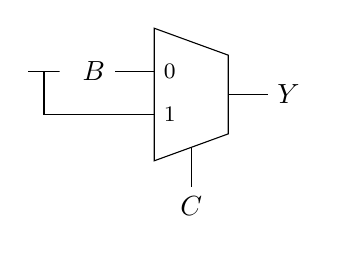
\begin{tikzpicture}[circuit ee IEC,small circuit symbols]

% Draw mux body.
\draw
    (0,0) coordinate (O)
    -- ++ (20:1) coordinate (A)
    -- ++ (90:1) coordinate (B)
    -- ++ (160:1) coordinate (C)
    -- cycle;

% Mux output.
\draw
    % Start in middle--this is so clever of tikz!
    ($(A)!0.5!(B)$)
    % draw right
    -- ++(0:5mm)
    % label output on right
    node[right]{$Y$};

% Mux input select.
\draw
    % start in the middle of lower mux body.
    ($(O)!0.50!(A)$)
    % draw down
    -- ++(270:5mm)
    % label C input select
    node[below]{$C$};

% Loop for each mux terminal.
\foreach \y/\t/\b in {0.1/0/0,0.2/1/1} {

    % Draw each terminal.
    \draw
        ($(C)! \y*3.25 !(O)$) -- ++(180:0.5cm)
        node(term\t)[anchor=center] {};

    % Draw binary numbers to select. End loop.
    \draw
        ($(C)! \y*3.25 !(O)$) ++ (0:0.0)
        node[right,font=\footnotesize] {$\b$};
}

% Draw the VDD symbol to input term0.
\draw
    % start at term0 center
    (term1.center)
    % these are for some adjustments since we're
    % using this picture as a template.
    -- ++(180:-0.0cm) -- ++(180:9mm)
    % go down
    -- ++(90:5.4mm)
    -- ++(0:2mm) -- ++(180:4mm);
    % ground symbol
    %node[ground={pos=1},point down]{};

% Draw B input on term1
\draw
    % start at term1 center
    (term0.center)
    % go down 0.5 cm.
    -- ++(0:-0.0mm)
    % label B on left.
    node[left]{$B$};

\end{tikzpicture}
\end{document}
